    \begin{figure}[H]
        \centering
        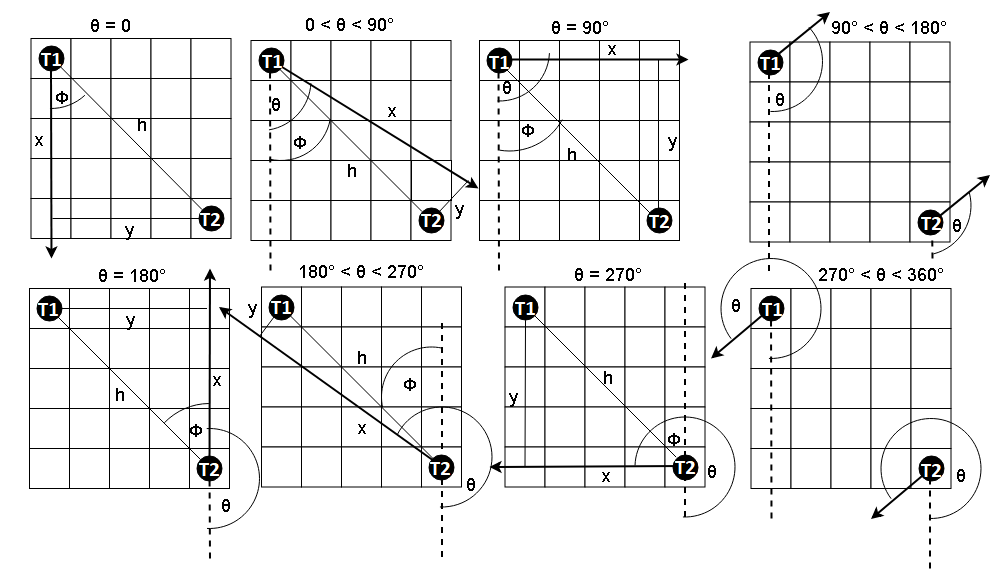
\includegraphics[width=\linewidth]{Figures/bestSmall.png}
        \caption{Schematics of a best configuration of a 1km by 1km wind farm with two wind turbines located at $(0,0)$ and $(4,4)$ for different wind directions.}
        \label{bestSmall}
    \end{figure}

Note that the distance between the two wind turbines can be solved using their position on the matrix. using the example above, by distance formula where $(i_{1},j_{1})$ is the position of the first wind turbine and $(i_{2},j_{2})$ is the position of the second wind turbine and also considering that each cell in the matrix have $200mx200m$ dimension,
    \begin{align*}
        h &= 200m\cdot \sqrt{(i_{2}+i_{1})^{2}+(j_{2}+j_{1})^{2}}\\
         &= 200m\cdot \sqrt{(4+0)^{2}+(4+0)^{2}} \\
         &= 200m\cdot \sqrt{4^{2}+4^{2}} \\
         &= 200m(5.6568) \\
         &= 1131.3708\;meters
    \end{align*}
Where h is the distance between the two wind turbines. Now that the actual distance between the wind turbine is determined, the length of the two legs of the right triangle formed by the wind direction and the $h$ as the hypotenuse is solved. Using the given figure, the $\theta=0^{o}$ and $\phi=45^{o}$ where the $\theta$ is the angle of the wind direction and $\phi$ is the angle from the reference point of the first wind turbine to $h$,the $x$ is solved by
    \begin{align*}
        x &= h(cos|(\theta\;mod\;90^{o})-\phi|) \\
          &= 1137.37m(cos|0^{o}-45^{o}|) \\
          &= (1137.37m)(0.7071) \\
        x &= 800m
    \end{align*}
and the $y$ is
    \begin{align*}
        y &= h(sin|(\theta\;mod\;90^{o})-\phi|) \\
          &= h(1137.37m)(0.7071) \\
        y  &= 800m
    \end{align*}
Since the $x=800m$, the resulting radius of the wake of the first wind turbine, $T_{1}$ is
    \begin{align*}
        r(x)   &= ax + r_{o} \\
        r(800) &= (0.3267545)(800m) + 20m \\
        r(800) &= 281.436m
    \end{align*}
where $a$ is the axial induction factor and $r_{0}$ is the rotor radius of the wind turbine. Since $y>r$, the wake of the first wind turbine will not affect the second wind turbine thus there is no wake interaction between the two turbines. Therefore the total power of both turbines using $u_{\infty}=12m/s$ as the wind speed is
    \begin{align*}
        P_{tot} &= P_{1} + P_{2} = 0.3u_{\infty}^{3} + 0.3u_{\infty}^{3} \\
        P_{tot} &= 0.3(12m/s)^{3} + 0.3(12m/s)^{3} \\
        P_{tot} &= 518.4kW + 518.4kW\\
        P_{tot} &= 1036.8kW
    \end{align*}
    
Now we consider if the wind directions is $0<\theta<90^{o}$. The position of the $x$ and $y$ will change and so is their length. Below shows the length of $x$ and $y$
different wind direction at $0<\theta<90$   
    \begin{align*}
        x_{\theta=10^{o}} = x_{\theta=80^{o}} &= (1131.37m)cos|10^{o}-45^{o}| &= 926.765m \\ 
        x_{\theta=20^{o}} = x_{\theta=70^{o}} &= (1131.37m)cos|20^{o}-45^{o}| &= 1025.370m \\ 
        x_{\theta=30^{o}} = x_{\theta=60^{o}} &= (1131.37m)cos|30^{o}-45^{o}| &= 1092.820m \\ 
        x_{\theta=40^{o}} = x_{\theta=50^{o}} &= (1131.37m)cos|40^{o}-45^{o}| &= 1127.066m \\ 
    \end{align*}
    with their respective $y$
    \begin{align*}
        y_{\theta=10^{o}} = y_{\theta=80^{o}} &= (1131.37m)sin|10^{o}-45^{o}| &= 648.928m \\ 
        y_{\theta=20^{o}} = y_{\theta=70^{o}} &= (1131.37m)sin|20^{o}-45^{o}| &= 473.138m \\ 
        y_{\theta=30^{o}} = y_{\theta=60^{o}} &= (1131.37m)sin|30^{o}-45^{o}| &= 292.820m \\ 
        y_{\theta=40^{o}} = y_{\theta=50^{o}} &= (1131.37m)sin|40^{o}-45^{o}| &= 98.605m \\ 
    \end{align*}
Computing the resulting radii of the wake at the given distances $x$, we have
    \begin{align*}
        r(x=926.765m) &= (0.3267949)(926.765m)+20m=322.8621m \\
        r(x=1025.370m) &= (0.3267949)(1025.370m)+20m=355.0857m \\
        r(x=1092.820m) &= (0.3267949)(1092.820m)+20m=377.1280m \\
        r(x=1127.066m) &= (0.3267949)(1127.066m)+20m=388.3194m \\
    \end{align*}
%%%
Note that the $y$ is greater than the resulting radius of the wake except at $\theta=30^{o},60^{O}$.
	\begin{align*}
		r(926.765m) &= 322.862 < y_{\theta=10^{o}|80^{o}} \\
		r(1025/370m) &= 355.086 < y_{\theta=20^{o}|70^{o}} \\
		r(1092.820m) &= 377.128 > y_{\theta=30^{o}|60^{o}} \\
		r(1127.066m) &= 388.819 > y_{\theta=50^{o}|50^{o}} 
	\end{align*}
This means that at $\theta=30^{o},60^{o},40^{o},50^{o} $ and , the wake of the first turbine will affect the second turbine, resulting in lower total power output.
%paki lagay nalang ung power output nung theta=30,60



%figure nang theta = 90

From the figure, the distance between the two turbine with respect to the wind direction is the same as the diffrence with the column position and row position. This means that $x$ is
	\begin{align*}
		x &= 1131.371m(cos|\theta-\phi|) \\
		  &= 1131.371m(cos|90^{o}-45^{o}|) \\
		  &= 1131.371m(cos|45^{o}|) \\
		  &= 800m	
	\end{align*}
and $y$ is 
	\begin{align*}
		y &= 1131.371m(sin|\theta-\phi|) \\
		  &= 1131.371m(sin|90^{o}-45^{o}|) \\
		  &= 1131.371m(sin|45^{o}|) \\
		  &= 800m	
	\end{align*}

Since the $x$ and $y$ is the same as if $\theta=0^{o}$, then the total power output is the same.

%figure nang theta 90 < theta < 180

Note that at $90^{o}<\theta<180^{o}$ wind direction, the $x$ and $y$ is computed as 
	\begin{align*}
		x_{\theta=100^{o}} &= 1131.371m(cos|100^{o}-45^{o}|) &= 926.765m &= x_{\theta=170^{o}} \\
	 	x_{\theta=110^{o}} &= 1131.371m(cos|110^{o}-45^{o}|) &= 1025.370m &= x_{\theta=160^{o}} \\
		x_{\theta=120^{o}} &= 1131.371m(cos|120^{o}-45^{o}|) &= 1092.820m &= x_{\theta=150^{o}} \\
		x_{\theta=130^{o}} &= 1131.371m(cos|130^{o}-45^{o}|) &= 1127.066m &= x_{\theta=140^{o}} \\
	\end{align*}
with their respective $y$ 
	\begin{align*}
		y_{\theta=100^{o}} &= 1131.371m(sin|100^{o}-45^{o}|) &= 648.928m &= y_{\theta=170^{o}} \\
	 	y_{\theta=110^{o}} &= 1131.371m(sin|110^{o}-45^{o}|) &= 478.138m &= y_{\theta=160^{o}} \\
		y_{\theta=120^{o}} &= 1131.371m(sin|120^{o}-45^{o}|) &= 292.820m &= y_{\theta=150^{o}} \\
		y_{\theta=130^{o}} &= 1131.371m(sin|130^{o}-45^{o}|) &=  98.605m &= y_{\theta=140^{o}} 
	\end{align*}

From the previous data, at $\theta=120^{o},150^{o}$ the $x$ and $y$ is the same at $\theta=30^{o},60^{o}$ and $\theta=130^{o},140^{o}$ is the same as $\theta=40^{o},50^{o}$. This means that the wake from the second turbine will affect the first turbine, resulting in lower total power output similar at $\theta=30^{o},60^{o}$ and $\theta=40^{o},50^{o}$.

%%%



This implies that there are wake interactions between the wind turbines at wind directions $\theta=30^o$, $\theta=40^o$, $\theta=50^o$ and $\theta=60^o$.

%%%%%%%%%%%%%%%%%%%%%%%%%%%%%%%%%%%%%%%%%%%%
Since the configuration is symmetric along a diagonal axis, the computation of power output for the wind turbines for wind directions from $\theta=180^o$ up to $\theta=360^o$ would be the same for wind directions $\theta=0^o$ up to $\theta=180^o$ except that their output shall interchange. The summary of the computation of $x$, $y$, the resulting radius of the wake $r$, wind speed at each wind turbine $u_1$ $u_1$, and the power output of each wind turbine $P_1$ $P_1$ are shown in Table \ref{summaryBest2}.

\singlespacing
\begin{table}[H]
    \centering
    \begin{tabular}{|c|c|c|c|c|c|c|c|} \hline
$\theta$ &$x$ &$y$ &$r$ &$u_1$ &$u_2$ &$P_1$ &$P_2$ \\ \hline
$0^o$	&800.0000	&800.0000	&281.4359	&12.0000	&12.0000	&518.4000	&518.4000 \\ \hline
$10^o$	&926.7647	&648.9277	&322.8620	&12.0000	&12.0000	&518.4000	&518.4000 \\ \hline
$20^o$	&1025.3702	&478.1380	&355.0858	&12.0000	&12.0000	&518.4000	&518.4000 \\ \hline
$30^o$	&1092.8203	&292.8203	&377.1281	&11.6448	&12.0000	&473.7131	&518.4000 \\ \hline
$40^o$	&1127.0656	&98.6055	&388.3193	&11.6617	&12.0000	&475.7782	&518.4000 \\ \hline
$50^o$	&1127.0656	&98.6055	&388.3193	&11.6617	&12.0000	&475.7782	&518.4000 \\ \hline
$60^o$	&1092.8203	&292.8203	&377.1281	&11.6448	&12.0000	&473.7131	&518.4000 \\ \hline
$70^o$	&1025.3702	&478.1380	&355.0858	&12.0000	&12.0000	&518.4000	&518.4000 \\ \hline
$80^o$	&926.7647	&648.9277	&322.8620	&12.0000	&12.0000	&518.4000	&518.4000 \\ \hline
$90^o$	&800.0000	&800.0000	&281.4359	&12.0000	&12.0000	&518.4000	&518.4000 \\ \hline
$100^o$	&926.7647	&648.9277	&322.8620	&12.0000	&12.0000	&518.4000	&518.4000 \\ \hline
$110^o$	&1025.3702	&478.1380	&355.0858	&12.0000	&12.0000	&518.4000	&518.4000 \\ \hline
$120^o$	&1092.8203	&292.8203	&377.1281	&12.0000	&12.0000	&518.4000	&518.4000 \\ \hline
$130^o$	&1127.0656	&98.6055	&388.3193	&12.0000	&12.0000	&518.4000	&518.4000 \\ \hline
$140^o$	&1127.0656	&98.6055	&388.3193	&12.0000	&12.0000	&518.4000	&518.4000 \\ \hline
$150^o$	&1092.8203	&292.8203	&377.1281	&12.0000	&12.0000	&518.4000	&518.4000 \\ \hline
$160^o$	&1025.3702	&478.1380	&355.0858	&12.0000	&12.0000	&518.4000	&518.4000 \\ \hline
$170^o$	&926.7647	&648.9277	&322.8620	&12.0000	&12.0000	&518.4000	&518.4000 \\ \hline
$180^o$	&800.0000	&800.0000	&281.4359	&12.0000	&12.0000	&518.4000	&518.4000 \\ \hline
$190^o$	&926.7647	&648.9277	&322.8620	&12.0000	&12.0000	&518.4000	&518.4000 \\ \hline
$200^o$	&1025.3702	&478.1380	&355.0858	&12.0000	&12.0000	&518.4000	&518.4000 \\ \hline
$210^o$	&1092.8203	&292.8203	&377.1281	&12.0000	&11.6448	&518.4000	&473.7131 \\ \hline
$220^o$	&1127.0656	&98.6055	&388.3193	&12.0000	&11.6617	&518.4000	&475.7782 \\ \hline
$230^o$	&1127.0656	&98.6055	&388.3193	&12.0000	&11.6617	&518.4000	&475.7782 \\ \hline
$240^o$	&1092.8203	&292.8203	&377.1281	&12.0000	&11.6448	&518.4000	&473.7131 \\ \hline
$250^o$	&1025.3702	&478.1380	&355.0858	&12.0000	&12.0000	&518.4000	&518.4000 \\ \hline
$260^o$	&926.7647	&648.9277	&322.8620	&12.0000	&12.0000	&518.4000	&518.4000 \\ \hline
$270^o$	&800.0000	&800.0000	&281.4359	&12.0000	&12.0000	&518.4000	&518.4000 \\ \hline
$280^o$	&926.7647	&648.9277	&322.8620	&12.0000	&12.0000	&518.4000	&518.4000 \\ \hline
$290^o$	&1025.3702	&478.1380	&355.0858	&12.0000	&12.0000	&518.4000	&518.4000 \\ \hline
$300^o$	&1092.8203	&292.8203	&377.1281	&12.0000	&12.0000	&518.4000	&518.4000 \\ \hline
$310^o$	&1127.0656	&98.6055	&388.3193	&12.0000	&12.0000	&518.4000	&518.4000 \\ \hline
$320^o$	&1127.0656	&98.6055	&388.3193	&12.0000	&12.0000	&518.4000	&518.4000 \\ \hline
$330^o$	&1092.8203	&292.8203	&377.1281	&12.0000	&12.0000	&518.4000	&518.4000 \\ \hline
$340^o$	&1025.3702	&478.1380	&355.0858	&12.0000	&12.0000	&518.4000	&518.4000 \\ \hline
$350^o$	&926.7647	&648.9277	&322.8620	&12.0000	&12.0000	&518.4000	&518.4000 \\ \hline
    \end{tabular}
    \caption{Summary of the computation of $x$, $y$, the resulting radius of the wake $r$, wind speed at each wind turbine $u_1$ $u_1$, and the power output of each wind turbine $P_1$ $P_1$ of two wind turbines located at $(0,0)$ and $(4,4)$ respectively on a 1km by 1km wind farm.}
    \label{summaryBest2}
\end{table}
\doublespacing

Since each wind direction's existence throughout the year is even, the fraction of occurrence of each wind direction is $\frac{1}{36}$. Therefore, the total annual power output of the whole wind farm with the current configuration would be
\begin{align*}
    P_{tot}
    &= \sum_{\theta=0^o}^{350^o} \left( P_{1[\theta]} + P_{2[\theta]} \right) \cdot \frac{1}{36} \\
    &= \frac{1}{36}\left( P_{1[\theta=0^o]} + P_{2[\theta=0^o]} \right) + \frac{1}{36}\left( P_{1[\theta=10^o]} + P_{2[\theta=10^o]} \right) +...+ \frac{1}{36}\left( P_{1[\theta=350^o]} + P_{2[\theta=350^o]} \right) \\
    &= \frac{1}{36}\cdot\left( 518.4kW + 518.4kW \right) + \frac{1}{36}\cdot\left( 518.4kW + 518.4kW \right) +...+ \frac{1}{36}\cdot\left( 518.4kW + 518.4kW \right) \\
    &=1027.0990kW
\end{align*}

\subsection{Worst Configuration of Two Wind Turbines}
    However, the worst configurations of the wind farm found by the exhaustive search are where the turbines are adjacent to each other horizontally and vertically for the two turbines have the shortest possible distance between them.
    
    \begin{figure}[H]
        \centering
        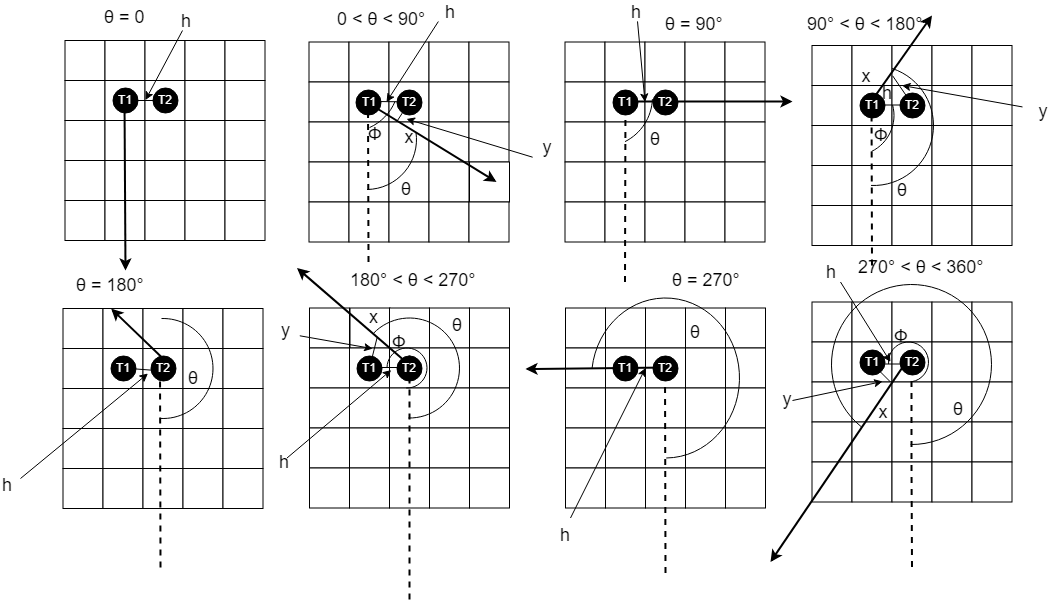
\includegraphics[width=\linewidth]{Figures/worstSmall.png}
        \caption{Schematics of a worst configuration of a 1km by 1km wind farm with two wind turbines located at $(1,1)$ and $(1,2)$ for different wind directions.}
        \label{worstSmall}
    \end{figure}
    
    Consider an example shown in Figure \ref{worstSmall} where the wind turbines $T_1$ and $T_2$ are located at $(1,1)$ and $(1,2)$ respectively with wind speed of $12m/s$ for every direction, the shortest distance between them $h$ is
    \begin{align*}
        h
        &=200m\cdot \sqrt{(1-1)^2 + (1-2)^2} \\
        &=200\;meters
    \end{align*}
    
    For wind directions $\theta=0^o$ as shown in Figure \ref{worstSmall}, the distance the two wind turbines with respect to the wind speed is $x=0$ while $y$ would be the same as $h$ by inspecting the figure. However, using our formula for x and y, the values would be the same as shown below.
    \begin{align*}
        \phi
    	&= tan^{-1} \left| \frac{1-2}{1-1} \right| \\
    	&= \lim_{\delta -> 0} \left( tan^{-1} \frac{1}{\delta} \right) \\
    	&= 90^o
    \end{align*}
        \begin{align*}
        x &= h(cos|(\theta\;mod\;90^{o})-\phi|) \\
          &= 200m(cos|0^{o}-90^{o}|) \\
          &= (200m)(0) \\
        x &= 0\;meters
    \end{align*}
and the $y$ is
    \begin{align*}
        y &= h(sin|(\theta\;mod\;90^{o})-\phi|) \\
          &= 200m(cos|0^{o}-90^{o}|) \\
          &= (200m)(1) \\
        y &= 200\;meters
    \end{align*}
    
    The resulting radius of the wake at a distance of $x=0\;meters$ would be
    \begin{align*}
        r(x=0)&=(0.3267949)(0) + 20m \\
        &= 20 \;meters
    \end{align*}
    which is less than $y$ which implies that there is no wake interaction between the two wind turbines at that wind direction. Therefore, the power output of each wind turbine $P_1$ and $P_2$ is
    \begin{align*}
        P_1=P_2
        &=0.3(12m/s)^3 \\
        &= 518.4kW
    \end{align*}
    
    The summary of the computation of $x$, $y$, the resulting radius of the wake $r$, wind speed at each wind turbine $u_1$ $u_1$, and the power output of each wind turbine $P_1$ $P_1$ for the given worst configuration of the wind farm with two wind turbines are shown in Table \ref{summaryWorst2}.
    
    \singlespacing
\begin{table}[H]
    \centering
    \begin{tabular}{|c|c|c|c|c|c|c|c|} \hline
$\theta$ &$x$ &$y$ &$r$ &$u_1$ &$u_2$ &$P_1$ &$P_2$ \\ \hline
$0^o$	&0.0000	&200.0000	&20.0000	&12.0000	&12.0000	&518.4000	&518.4000 \\ \hline
$10^o$	&34.7296	&196.9616	&31.3495	&12.0000	&12.0000	&518.4000	&518.4000 \\ \hline
$20^o$	&68.4040	&187.9385	&42.3541	&12.0000	&12.0000	&518.4000	&518.4000 \\ \hline
$30^o$	&100.0000	&173.2051	&52.6795	&12.0000	&12.0000	&518.4000	&518.4000 \\ \hline
$40^o$	&128.5575	&153.2089	&62.0119	&12.0000	&12.0000	&518.4000	&518.4000 \\ \hline
$50^o$	&153.2089	&128.5575	&70.0679	&12.0000	&12.0000	&518.4000	&518.4000 \\ \hline
$60^o$	&173.2051	&100.0000	&76.6025	&12.0000	&12.0000	&518.4000	&518.4000 \\ \hline
$70^o$	&187.9385	&68.4040	&81.4174	&9.0701	&12.0000	&223.8486	&518.4000 \\ \hline
$80^o$	&196.9616	&34.7296	&84.3660	&9.1765	&12.0000	&231.8188	&518.4000 \\ \hline
$90^o$	&200.0000	&0.0000	&85.3590	&9.2110	&12.0000	&234.4453	&518.4000 \\ \hline
$100^o$	&34.7296	&196.9616	&31.3495	&12.0000	&12.0000	&518.4000	&518.4000 \\ \hline
$110^o$	&68.4040	&187.9385	&42.3541	&12.0000	&12.0000	&518.4000	&518.4000 \\ \hline
$120^o$	&100.0000	&173.2051	&52.6795	&12.0000	&12.0000	&518.4000	&518.4000 \\ \hline
$130^o$	&128.5575	&153.2089	&62.0119	&12.0000	&12.0000	&518.4000	&518.4000 \\ \hline
$140^o$	&153.2089	&128.5575	&70.0679	&12.0000	&12.0000	&518.4000	&518.4000 \\ \hline
$150^o$	&173.2051	&100.0000	&76.6025	&12.0000	&12.0000	&518.4000	&518.4000 \\ \hline
$160^o$	&187.9385	&68.4040	&81.4174	&9.0701	&12.0000	&223.8486	&518.4000 \\ \hline
$170^o$	&196.9616	&34.7296	&84.3660	&9.1765	&12.0000	&231.8188	&518.4000 \\ \hline
$180^o$	&0.0000	&200.0000	&20.0000	&12.0000	&12.0000	&518.4000	&518.4000 \\ \hline
$190^o$	&34.7296	&196.9616	&31.3495	&12.0000	&12.0000	&518.4000	&518.4000 \\ \hline
$200^o$	&68.4040	&187.9385	&42.3541	&12.0000	&12.0000	&518.4000	&518.4000 \\ \hline
$210^o$	&100.0000	&173.2051	&52.6795	&12.0000	&12.0000	&518.4000	&518.4000 \\ \hline
$220^o$	&128.5575	&153.2089	&62.0119	&12.0000	&12.0000	&518.4000	&518.4000 \\ \hline
$230^o$	&153.2089	&128.5575	&70.0679	&12.0000	&12.0000	&518.4000	&518.4000 \\ \hline
$240^o$	&173.2051	&100.0000	&76.6025	&12.0000	&12.0000	&518.4000	&518.4000 \\ \hline
$250^o$	&187.9385	&68.4040	&81.4174	&12.0000	&9.0701	&518.4000	&223.8486 \\ \hline
$260^o$	&196.9616	&34.7296	&84.3660	&12.0000	&9.1765	&518.4000	&231.8188 \\ \hline
$270^o$	&200.0000	&0.0000	&85.3590	&12.0000	&9.2110	&518.4000	&234.4453 \\ \hline
$280^o$	&34.7296	&196.9616	&31.3495	&12.0000	&12.0000	&518.4000	&518.4000 \\ \hline
$290^o$	&68.4040	&187.9385	&42.3541	&12.0000	&12.0000	&518.4000	&518.4000 \\ \hline
$300^o$	&100.0000	&173.2051	&52.6795	&12.0000	&12.0000	&518.4000	&518.4000 \\ \hline
$310^o$	&128.5575	&153.2089	&62.0119	&12.0000	&12.0000	&518.4000	&518.4000 \\ \hline
$320^o$	&153.2089	&128.5575	&70.0679	&12.0000	&12.0000	&518.4000	&518.4000 \\ \hline
$330^o$	&173.2051	&100.0000	&76.6025	&12.0000	&12.0000	&518.4000	&518.4000 \\ \hline
$340^o$	&187.9385	&68.4040	&81.4174	&12.0000	&9.0701	&518.4000	&223.8486 \\ \hline
$350^o$	&196.9616	&34.7296	&84.3660	&12.0000	&9.1765	&518.4000	&231.8188 \\ \hline
    \end{tabular}
    \caption{Summary of the computation of $x$, $y$, the resulting radius of the wake $r$, wind speed at each wind turbine $u_1$ $u_1$, and the power output of each wind turbine $P_1$ $P_1$ of two wind turbines located at $(1,1)$ and $(1,2)$ respectively on a 1km by 1km wind farm.}
    \label{summaryWorst2}
\end{table}
\doublespacing

Since each wind direction's existence throughout the year is even, the fraction of occurrence of each wind direction is $\frac{1}{36}$. Therefore, the total annual power output of the whole wind farm with the current configuration would be
\begin{align*}
    P_{tot}
    &= \sum_{\theta=0^o}^{350^o} \left( P_{1[\theta]} + P_{2[\theta]} \right) \cdot \frac{1}{36} \\
    &= \frac{1}{36}\left( P_{1[\theta=0^o]} + P_{2[\theta=0^o]} \right) + \frac{1}{36}\left( P_{1[\theta=10^o]} + P_{2[\theta=10^o]} \right) +...+ \frac{1}{36}\left( P_{1[\theta=350^o]} + P_{2[\theta=350^o]} \right) \\
    &= \frac{1}{36}\cdot\left( 518.4kW + 518.4kW \right) + \frac{1}{36}\cdot\left( 518.4kW + 518.4kW \right) +...+ \frac{1}{36}\cdot\left( 518.4kW + 281.8kW \right) \\
    &=956.4545kW
\end{align*}